\documentclass[tikz,border=1pt]{standalone}
\begin{document}
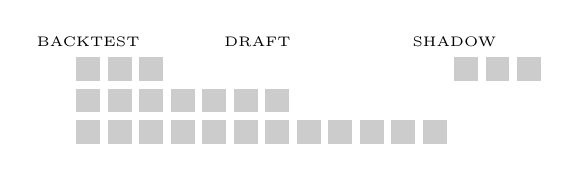
\begin{tikzpicture}
    \foreach \x/\y in {0/0,1/0,2/0,12/0,13/0,14/0,0/1,1/1,2/1,3/1,4/1,5/1,6/1,0/2,1/2,2/2,3/2,4/2,5/2,6/2,7/2,8/2,9/2,10/2,11/2} {
        \fill[gray!40] (\x*0.4,-\y*0.4) rectangle (\x*0.4+0.3,-\y*0.4+0.3);
    }
    \node[font=\tiny] at (0.15,0.5) {BACKTEST};
    \node[font=\tiny] at (2.3,0.5) {DRAFT};
    \node[font=\tiny] at (4.8,0.5) {SHADOW};
\end{tikzpicture}
\end{document}
